\section[Fonctions de perte, Optimisation et Initialisation]{Fonctions de perte, Optimisation et Initialisation}

\begin{frame}{Fonctions de perte, Optimisation et Initialisation}
	Maintenant que l'algorithme de la rétro-propagation du gradient n'a plus de secrets pour vous, il nous reste à nous attaquer à trois aspects que nous avons mis de côté pour l'instant:
	
	\begin{itemize}
		\item Les \textbf{fonctions de perte}: nous avons propagé le gradient d'une erreur $\delta$ mais sans dire encore comment on le calculait.
		\pause
		\item L'\textbf{optimisation}: on a brièvement discuté comment \textit{mettre à jour} les termes de poids et de biais une fois qu'on a obtenu les gradients en faisant une descente de gradient, mais il nous reste encore beaucoup à dire sur l'optimisation.
		\pause
		\item L'\textbf{initialisation}: nous sommes restés très évasifs sur l'initialisation des poids et des biais. On a admis qu'ils sont initialisés \textit{aléatoirement}. On verra \textit{précisément} comment cette initialisation peut être réalisée.
	\end{itemize}
\end{frame}

\subsection[Fonctions de perte]{Fonctions de perte}

\begin{frame}{Fonctions de perte}
	Dans cette section on présentera quelques fonctions de perte pour les problèmes d'apprentissage supervisés que nous avons rencontrés jusqu'à présent:
	\begin{itemize}
		\item Pour les problèmes de régression linéaire: la fonction des \textbf{erreurs quadratiques}.
		\item Pour les problèmes de classification binaire: la fonction d'\textbf{entropie croisée binaire}.
		\item Pour les problèmes de classification multi-classe: la fonction d'\textbf{entropie croisée}.
	\end{itemize}
	Il nous faudra également introduire la méthode pour alimenter la rétro-propagation du gradient en calculant les dérivées de ces fonctions de perte.
\end{frame}

\begin{frame}{Précision de convention de nommage}
	\begin{itemize}
		\item La \textbf{fonction de perte} $L$ permet de calculer une erreur unitaire, pour une observation.
		\item La \textbf{fonction de coût} permet d'agréger les fonctions de perte pour l'ensemble des observations. L'opération d'agrégation la plus courante est la moyenne. Dans notre introduction, nous avons appelé cette fonction risque empirique $R_n$.
		\item L'\textbf{erreur} $e$ est un scalaire pour l'ensemble des $n$ observations, c'est le résultat de la fonction de coût.
	\end{itemize}
	\vspace{0.5cm}
	\begin{equation*}
		e = \frac{1}{n} \sum_{i=1}^{n} L\left(y^{(i)}, \hat{y}^{(i)}\right)
	\end{equation*}
\end{frame}

\subsection[Fonction de perte pour la régression]{Fonction de perte pour la régression}

\begin{frame}{Erreurs quadratiques pour la régression}
	La fonction des erreurs quadratiques a déjà été introduite dans le chapitre 1 sur les bases de l'apprentissage:
	\begin{equation*}
		L\left(y^{(i)}, \hat{y}^{(i)}\right) = \left(y^{(i)} - \hat{y}^{(i)}\right)^2
	\end{equation*}
	C'est la fonction de perte que nous avons utilisée pour la régression linéaire.
	\pause
	\begin{equation*}
		e = \frac{1}{n} \sum_{i=1}^n \left(y^{(i)} - \hat{y}^{(i)}\right)^2
	\end{equation*}
	\pause
	Le gradient $\delta = \frac{\partial{e}}{\partial{\hat{Y}}} \in \mathcal{M}_{n,1}(\R)$ peut être calculé comme suit:
	\begin{equation*}
		\delta = 
		\begin{pmatrix}
			\frac{\partial{e}}{\partial{\hat{y}^{(1)}}} \\[5pt]
			\frac{\partial{e}}{\partial{\hat{y}^{(2)}}} \\[5pt]
			\vdots \\
			\frac{\partial{e}}{\partial{\hat{y}^{(n)}}} \\
		\end{pmatrix}
		=
		\begin{pmatrix}
			\frac{2}{n} \left(\hat{y}^{(1)} - y^{(1)}\right) \\
			\frac{2}{n} \left(\hat{y}^{(2)} - y^{(2)}\right) \\
			\vdots \\
			\frac{2}{n} \left(\hat{y}^{(n)} - y^{(n)}\right)
		\end{pmatrix}
		= \frac{2}{n} \left(\hat{Y} - Y\right)
	\end{equation*}
\end{frame}

\begin{frame}{Fonction de perte pour un problème de régression}
	\begin{block}{Fonction de perte pour un problème de régression}
		Pour un problème de régression avec les sorties $Y \in \mathcal{M}_{n,1}(\R)$ et les prédictions du réseau de neurones $\hat{Y} \in \mathcal{M}_{n,1}(\R)$, on peut calculer l'erreur $e \in \R$ pour $n$ observations comme suit:
		\begin{equation*}
			e = \frac{1}{n} \sum_{i=1}^n \left(y^{(i)} - \hat{y}^{(i)}\right)^2 = \frac{1}{n} \left(Y - \hat{Y}\right)^T \left(Y - \hat{Y}\right)
		\end{equation*}
		Le gradient de cette erreur $e$ en fonction des prédictions $\hat{Y}$ s'écrit:
		\begin{equation*}
			\frac{\partial{e}}{\partial{\hat{Y}}} = \frac{2}{n} \left(\hat{Y} - Y\right)
		\end{equation*}
		Cette erreur est souvent appelée \textbf{erreur quadratique moyenne} (Mean-Squared Error (MSE)).
	\end{block}
\end{frame}

\subsection[Fonction de perte pour la classification binaire]{Fonction de perte pour la classification binaire}

\begin{frame}{Entropie croisée binaire}
	Nous avons déjà rencontré l'entropie croisée binaire à deux reprises dans le cours:
	\begin{itemize}
		\item Dans le premier cours lorsque nous avons introduit la fonction de perte pour la \textbf{régression logistique}.
		\item Dans le cours sur les arbres de décision. Nous avions alors utilisé l'entropie comme mesure de la \textit{pureté} d'une feuille.
	\end{itemize}
	\pause
	On a vu que l'entropie croisée consiste à évaluer la surprise moyenne pour notre réseau de neurones (la probabilité prédite) quand on le confronte aux données d'apprentissage (probabilités réelles). Minimiser l'entropie croisée consiste à minimiser les \textit{différences} entre la probabilité réelle (donné par les observations) et les probabilités prédites. Minimiser cette différence, c'est aussi minimiser la divergence de Kullback-Leibler comme on l'a vu dans le cours sur les arbres de décision.
\end{frame}

\begin{frame}{Entropie croisée binaire}
	Nous avons également discuté qu'il y avait néanmoins une différence fondamentale entre la définition de l'entropie croisée et de son application à l'apprentissage automatique:
	\begin{itemize}
		\item Dans la définition de l'entropie croisée on réalise $n$ expériences pour un sujet \textbf{unique}: pour un lancer de pièce dont on a estimé la probabilité de succès (résultat "Face"), on effectue plusieurs répétitions pour calculer une surprise moyenne (autrement dit, une entropie croisée).
		\item Dans l'application à l'apprentissage automatique: nous n'avons qu'\textbf{une} observation pour $n$ sujets \textbf{différents}. Il y a  autant de probabilités estimées et réelles que d'observations.
	\end{itemize}
	\pause
	Pour un problème de classification binaire la fonction de perte liée à l'entropie croisée s'écrit:
	\begin{equation*}
		L\left(y^{(i)}, \hat{y}^{(i)}\right) = - y^{(i)} \ln{\left(\hat{y}^{(i)}\right)} - \left(1 - y^{(i)}\right) \ln{\left(1 - \hat{y}^{(i)}\right)}
	\end{equation*}
\end{frame}

\begin{frame}{Entropie croisée binaire moyenne}
	On agrège les entropies croisées calculées pour l'ensemble des observations en un terme d'erreur $e$:
	\begin{equation*}
		e = \frac{1}{n} \sum_{i=1}^n - y^{(i)} \ln{\left(\hat{y}^{(i)}\right)} - \left(1 - y^{(i)}\right) \ln{\left(1 - \hat{y}^{(i)}\right)}
	\end{equation*}
	\pause
	Le gradient $\delta = \frac{\partial{e}}{\partial{\hat{Y}}} \in \mathcal{M}_{n,1}(\R)$ peut être calculé comme suit:
	\begin{equation*}
		\begin{aligned}
			\delta 
			&= 
			\begin{pmatrix}
				\frac{\partial{e}}{\partial{\hat{y}^{(1)}}} \\[5pt]
				\frac{\partial{e}}{\partial{\hat{y}^{(2)}}} \\[5pt]
				\vdots \\
				\frac{\partial{e}}{\partial{\hat{y}^{(n)}}} \\
			\end{pmatrix}
			= \frac{1}{n}
			\begin{pmatrix}
				-\frac{y^{(1)}}{\hat{y}^{(1)}} + \frac{\left(1 - y^{(1)}\right)}{\left(1 - \hat{y}^{(1)}\right)} \\[5pt]
				-\frac{y^{(2)}}{\hat{y}^{(2)}} + \frac{\left(1 - y^{(2)}\right)}{\left(1 - \hat{y}^{(2)}\right)} \\[5pt]
				\vdots \\
				-\frac{y^{(n)}}{\hat{y}^{(n)}} + \frac{\left(1 - y^{(n)}\right)}{\left(1 - \hat{y}^{(n)}\right)}
			\end{pmatrix} \\
			&= \frac{1}{n} \left( -Y \oslash \hat{Y} + \left(1_Y - Y\right) \oslash \left(1_Y - \hat{Y}\right)\right)
		\end{aligned}
	\end{equation*}
\end{frame}

\begin{frame}{Optimisation de l'entropie croisée binaire pour la propagation des gradients}
	Il y a une optimisation généralement implémentée dans les bibliothèques traitant les réseaux de neurones:
	\begin{itemize}
		\item Pour un problème de classification binaire, une fonction \textbf{logistique} est utilisée pour transformer les \textbf{logits} en \textbf{probabilités}.
		\item Lors de la rétro-propagation du gradient à travers cette fonction logistique, la combinaison de la dérivée de l'entropie croisée binaire et de la dérivée de la fonction logistique conduit à une expression simplifiée.
	\end{itemize}
\end{frame}

\begin{frame}{Optimisation de l'entropie croisée binaire pour la propagation des gradients}
	La dérivée de la fonction logistique est:
	\begin{equation*}
		\sigma'(Z) = \sigma(Z) \odot \left(1_Z - \sigma(Z)\right) = \hat{Y} \odot (1_Y - \hat{Y})
	\end{equation*}
	\pause
	Par conséquent:
	\begin{equation*}
		\begin{aligned}
			\frac{\partial{e}}{\partial{Z}} 
			&= \delta \odot \sigma'(Z) \\
			&= \frac{1}{n} \left( - Y \oslash \hat{Y} + \left(1_Y - Y\right) \oslash \left(1_Y - \hat{Y}\right)\right) \odot \hat{Y} \odot (1_Y - \hat{Y}) \\
			&= \frac{1}{n} \left( - Y \odot (1_Y - \hat{Y}) + \hat{Y} \left(1_Y - Y\right)\right) \\
			&= \frac{1}{n} \left( - Y + Y \odot \hat{Y} + \hat{Y} - \hat{Y} \odot Y \right) \\
			&= \frac{1}{n} \left( \hat{Y} -Y \right)
		\end{aligned}
	\end{equation*}
\end{frame}

\begin{frame}{Fonction de perte pour un problème de classification binaire}
	\begin{block}{Fonction de perte pour un problème de classification binaire}
		Pour un problème de classification binaire avec les sorties $Y \in \mathcal{M}_{n,1}(\{0, 1\})$, les \textbf{logits} prédits par le réseau de neurones $Z \in \mathcal{M}_{n,1}(\R)$ et $\sigma$ la fonction \textbf{logistique}, on peut calculer l'erreur $e \in \R$ pour $n$ observations comme suit:
		\begin{equation*}
			e = \frac{1}{n} \sum_{i=1}^n - y^{(i)} \ln{\left(\sigma\left(z^{(i)}\right)\right)} - \left(1 - y^{(i)}\right) \ln{\left(1 - \sigma\left(z^{(i)}\right)\right)}
		\end{equation*}
		Le gradient de cette erreur $e$ en fonction des logits $Z$ s'écrit:
		\begin{equation*}
			\frac{\partial{e}}{\partial{Z}} = \frac{1}{n} \left(\sigma\left(Z\right) - Y\right)
		\end{equation*}
		Cette fonction de perte qui combine la dernière fonction d'activation logistique et une entropie croisée binaire est appelée entropie croisée binaire à partir des logits (Binary Cross Entropy (BCE) with Logits).
	\end{block}
\end{frame}

\begin{frame}{Simplification d'un réseau de neurones pour de la classification binaire}
	Pour un problème de classification binaire, on peut simplifier l'architecture. Pour l'apprentissage:
	\begin{itemize}
		\item On n'utilise \textbf{pas} de fonction d'activation dans la couche de sortie. Le réseau de neurones calcule des \textbf{logits}.
		\pause
		\item La fonction de perte d'entropie croisée à partir des logits est utilisée. Techniquement, calculer l'erreur $e$ n'est pas nécessaire pour l'apprentissage, on peut directement calculer le gradient $\frac{\partial{e}}{\partial{Z}}$. C'est plus rapide et plus stable numériquement.
		\pause
		\item En pratique, on calcule tout de même l'erreur $e$ afin de contrôler la convergence de l'apprentissage.
	\end{itemize}
	
	\pause
	\vspace{0.3cm}
	
	Une fois le réseau de neurones entraîné, il ne faut pas oublier de rajouter une fonction logistique dans la couche de sortie afin que le réseau de neurones convertisse les \textbf{logits} en \textbf{probabilités}.
\end{frame}

\begin{frame}{Erreurs quadratiques vs entropie croisée pour la classification}
	En pratique, utiliser la fonction des erreurs quadratiques pour un problème de classification binaire \textit{fonctionne}. Après tout, on cherche à minimiser l'erreur d'une prédiction, et une probabilité est un nombre réel. Même si cela \textit{fonctionne}, c'est un choix non optimal:
	\begin{figure}
		\centering
		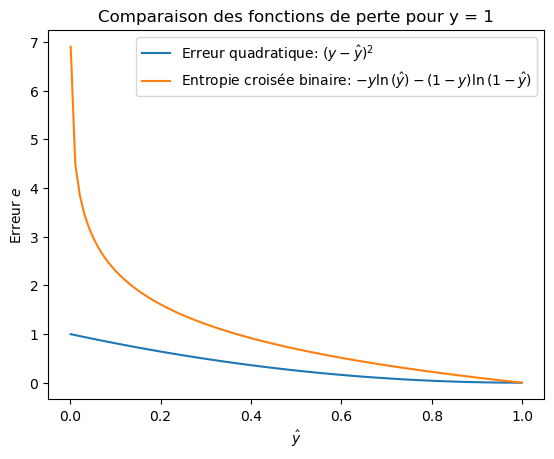
\includegraphics[width=0.4\linewidth]{Images/mse_vs_bce}
		\label{fig:mse_vs_bce}
	\end{figure}
	L'erreur augmente beaucoup plus rapidement avec l'entropie croisée qu'avec une erreur quadratique. Cela pénalise davantage le réseau de neurones qui classerait incorrectement l'observation.
\end{frame}

\subsection[Fonction de perte pour la classification multi-classe]{Fonction de perte pour la classification multi-classe}

\begin{frame}{$\hat{Y}$ et $Y$ dans un problème de classification multi-classe}
	Dans un problème de classification à $K$ classes, les probabilités prédites $\hat{Y}$ et les probabilités réelles $Y$ sont des matrices $\mathcal{M}_{n, K}([0, 1])$ avec $n$ le nombre d'observations.
	
	\pause
	\vspace{0.5cm}
	
	Pour chaque observation $i$, si la classe vraie est $k$, alors:
	
	\begin{equation*}
		\begin{cases}
			y_{j}^{(i)} = 1 & j = k \\
			y_{j}^{(i)} = 0 & j \ne k \\
		\end{cases} \; \text{ pour } \; j = 1, 2, \cdots, K
	\end{equation*}
	
	\vspace{0.5cm}
	
	C'est ce que l'on appelle l'encodage \textbf{One Hot}.
\end{frame}

\begin{frame}{Entropie croisée catégorielle dans un problème de classification à $K$ classes}
	Dans le cas général de la classification multi-classe, le concept est le même que précédemment:
	\begin{itemize}
		\item On remplace l'entropie croisée binaire par l'\textbf{entropie croisée catégorielle}.
		\pause
		\item On remplace la fonction logistique par l'activation \textbf{softmax}.
		\pause
		\item La fonction de perte inclura la fonction d'activation afin de stabiliser et d'accélérer l'algorithme d'apprentissage.
	\end{itemize}
\end{frame}

\begin{frame}{Entropie croisée catégorielle dans un problème de classification à $K$ classes}
	L'expression générale de l'entropie croisée catégorielle est:
	\begin{equation*}
		L\left(y^{(i)}, \hat{y}^{(i)}\right) = -\sum_{k=1}^K y_k^{(i)} \ln{\left(\hat{y}_k^{(i)}\right)}
	\end{equation*}
	\pause
	Si $K = 2$, on retrouve bien la même expression que l'entropie croisée binaire:
	\begin{equation*}
		\begin{aligned}
			L\left(y^{(i)}, \hat{y}^{(i)}\right) 
			&= -\sum_{k=1}^2 y_k^{(i)} \ln{\left(\hat{y}_k^{(i)}\right)}
			= - y_{1}^{(i)} \ln{\left(\hat{y}_{1}^{(i)}\right)} - y_{2}^{(i)} \ln{\left(\hat{y}_{2}^{(i)}\right)} \\
			&= - y_{1}^{(i)} \ln{\left(\hat{y}_{1}^{(i)}\right)} - \left(1 - y_{1}^{(i)}\right) \ln{\left(1 - \hat{y}_{1}^{(i)}\right)}
		\end{aligned}
	\end{equation*}
\end{frame}

\begin{frame}{Entropie croisée catégorielle moyenne}
	On agrège les entropies croisées catégorielles calculées pour l'ensemble des observations en un terme d'erreur $e$:
	\begin{equation*}
		e = \frac{1}{n} \sum_{i=1}^n \sum_{k=1}^K - y_k^{(i)} \ln{\left(\hat{y}_k^{(i)}\right)}
	\end{equation*}
	\pause
	Le gradient $\delta = \frac{\partial{e}}{\partial{\hat{Y}}} \in \mathcal{M}_{n,K}(\R)$ est la matrice suivante:
	\begin{equation*}
		\delta 
		= 
		\begin{pmatrix}
			\frac{\partial{e}}{\partial{\hat{y}_1^{(1)}}} & \frac{\partial{e}}{\partial{\hat{y}_2^{(1)}}} & \cdots & \frac{\partial{e}}{\partial{\hat{y}_K^{(1)}}} \\[5pt]
			\frac{\partial{e}}{\partial{\hat{y}_1^{(2)}}} & \frac{\partial{e}}{\partial{\hat{y}_2^{(2)}}} & \cdots & \frac{\partial{e}}{\partial{\hat{y}_K^{(2)}}}\\[5pt]
			\vdots & \vdots & \cdots & \vdots \\
			\frac{\partial{e}}{\partial{\hat{y}_1^{(n)}}} & \frac{\partial{e}}{\partial{\hat{y}_2^{(n)}}} & \cdots & 
			\frac{\partial{e}}{\partial{\hat{y}_K^{(n)}}}\\[5pt]
		\end{pmatrix}
	\end{equation*}
\end{frame}

\begin{frame}{Entropie croisée catégorielle moyenne}
	Les différents termes de ce gradient se calculent ainsi:
	\begin{equation*}
		\delta_{i,k} = \frac{\partial{e}}{\partial{\hat{Y}_{i,k}}} = - \frac{1}{n} \frac{y_k^{(i)}}{\hat{y}_k^{(i)}}
	\end{equation*}
	\pause
	En notation tensorielle:
	\begin{equation*}
		\delta = \frac{\partial{e}}{\partial{\hat{Y}}} = - \frac{1}{n} Y \oslash \hat{Y}
	\end{equation*}	
\end{frame}


\begin{frame}{Fonction d'activation softmax}
	On rappelle la définition de la fonction softmax sur la couche de sortie du réseau de neurones:
	\begin{equation*}
		\operatorname{softmax}(z_j) = \frac{e^{z_j}}{\sum_{k=1}^{K} e^{z_k}} \; \forall \; j = 1, 2, \cdots, K
	\end{equation*}
	\pause
	Par rapport aux fonctions d'activations que nous avions vu jusqu'à présent, il y a trois différences majeures:
	\begin{itemize}
		\item La sortie de cette fonction d'activation est maintenant une matrice de dimension $(n \times K)$.
		\item La sortie pour une observation $i$ et une classe $k$ est connectée à une seule observation $i$ mais à toutes les $K$ classes des entrées (c'est le terme de sommation au dénominateur).
		\item La dérivée de la fonction softmax par rapport à ses entrées est un tenseur $(n\times K \times n \times K)$.
	\end{itemize}
\end{frame}

\begin{frame}{Fonction d'activation softmax tensorielle}
	\begin{itemize}
		\item Le terme au dénominateur est la somme suivant les lignes d'un tenseur de dimension $(n \times K)$. Techniquement il s'agit d'un tenseur de dimension $(n, 1)$ que l'on peut écrire: $\exp{(Z)} 1_K$
		\pause
		\item Le terme au numérateur est un tenseur de dimension $(n \times K)$, c'est simplement: $\exp{(Z)}$
		\pause
		\item Le broadcasting des bibliothèques de calcul matriciel rend cette division d'un tenseur $(n \times K)$ par un tenseur $(1, K)$ possible. Mais pour rendre l'opération rigoureuse d'un point de vue mathématique on utilisera une petite astuce. En multipliant cette somme par $1_K^T$ cela permet de faire la même chose que le broadcasting: $\sum_{k=1}^{K} e^{z_k}$ devient alors $\exp{(Z)} 1_K 1_K^T$.
	\end{itemize}
	La notation tensorielle de la fonction softmax est donc:
	\begin{equation*}
		\operatorname{softmax}(Z) = \exp{(Z)} \oslash \left(\exp{(Z)} 1_K 1_K^T\right)
	\end{equation*}
\end{frame}

\begin{frame}{Dérivée de la fonction softmax tensorielle}
	La dérivée de la fonction softmax par rapport à ses entrées est un tenseur de dimension $(n\times K \times n \times K)$. Autant le dire tout de suite, on ne va pas s'amuser à le calculer. En fait, on va utiliser la même astuce que précédemment. On va passer par une \textbf{contraction tensorielle}.
	
	\vspace{0.5cm}
	
	Le résultat aboutit à la même chose que pour l'entropie croisée binaire moyenne combiné à une fonction logistique:
	
	\begin{equation*}
		\frac{\partial{e}}{\partial{Z}} = \frac{1}{n} \left(\hat{Y} - Y \right)
	\end{equation*}
	
	Ce résultat est démontré dans les annexes du cours.
	
\end{frame}

\begin{frame}{Fonction de perte pour un problème de classification multi-classe}
	\begin{block}{Fonction de perte pour un problème de classification multi-classe}
		Pour un problème de classification à $K$ classes avec les sorties $Y \in \mathcal{M}_{n,K}(\{0, 1\})$, les \textbf{logits} prédits par le réseau de neurones $Z \in \mathcal{M}_{n,K}(\R)$ et la fonction \textbf{softmax}, on peut calculer l'erreur $e \in \R$ pour $n$ observations comme suit:
		\begin{equation*}
			e = - \frac{1}{n} \sum_{i=1}^n \sum_{k=1}^K y_k^{(i)} \ln{\left(\hat{y}_k^{(i)}\right)}
		\end{equation*}
		Le gradient de cette erreur $e$ en fonction des logits $Z$ s'écrit:
		\begin{equation*}
			\frac{\partial{e}}{\partial{Z}} = \frac{1}{n} \left(\operatorname{softmax}\left(Z\right) - Y\right)
		\end{equation*}
	\end{block}
\end{frame}

\begin{frame}{Simplification d'un réseau de neurones pour de la classification multi-classe}
	Pour un problème de classification multi-classe, on peut simplifier l'architecture. Pour l'apprentissage:
	\begin{itemize}
		\item On n'utilise \textbf{pas} de fonction d'activation dans la couche de sortie. Le réseau de neurones calcule des \textbf{logits}.
		\pause
		\item La fonction de perte d'entropie croisée à partir des logits est utilisée. Techniquement, calculer l'erreur $e$ n'est pas nécessaire pour l'apprentissage, on peut directement calculer le gradient $\frac{\partial{e}}{\partial{Z}}$. C'est plus rapide et plus stable numériquement.
		\pause
		\item En pratique, on calcule tout de même l'erreur $e$ afin de contrôler la convergence de l'apprentissage.
	\end{itemize}
	
	\pause
	\vspace{0.3cm}
	
	Une fois le réseau de neurones entraîné, il ne faut pas oublier de rajouter une fonction softmax dans la couche de sortie afin que le réseau de neurones convertisse les \textbf{logits} en \textbf{probabilités}.
\end{frame}

\begin{frame}{Conclusions pour les fonctions de perte}
	Nous disposons maintenant de tout l'arsenal pour la rétro-propagation:
	\begin{itemize}
		\item En partant de la fonction de perte, dont la nature change en fonction du problème d'apprentissage supervisé, on a vu comment on pouvait calculer le \textbf{gradient de l'erreur} et le \textbf{propager} à travers la dernière couche d'activation.
		\pause
		\item Nous avions vu précédemment comment propager ce gradient à travers de l'ensemble des opérations que nous pouvons rencontrer dans notre réseau de neurones: \textbf{opérateur linéaire} et \textbf{fonction d'activation}.
		\pause
		\item Nous savons donc calculer le \textbf{gradient de l'erreur} en fonction de \textbf{tout paramètre} dans le réseau de neurones.
		\pause
		\item Il ne nous reste plus qu'à voir comment \textbf{initialiser} les paramètres du réseau de neurones et les \textbf{mettre à jour} pendant l'apprentissage.
	\end{itemize}
\end{frame}

\subsection[Minimisation par descente de gradient]{Minimisation par descente de gradient}

\begin{frame}{Rappel descente de gradient}
	On notera $P$ un paramètre quelconque du réseau de neurones. C'est un tenseur dans $\mathcal{M}_{u,v}(\R)$. Les paramètres de type biais ont $u = 1$.
	
	\vspace{0.3cm}
	\pause
	
	L'algorithme de descente de gradient peut être décrit comme suit:
	\begin{enumerate}
		\item Les paramètres sont initialisés: $P_{k=0}$
		\pause
		\item Boucle sur les époques jusqu'à ce qu'un critère d'arrêt soit rencontré (nombre d'époques maximum atteint, erreur sous un certain seuil, erreur ne diminuant plus,...)
		\pause
		\item Pour toutes les observations des données d'apprentissage:
		\begin{itemize}
			\item Calcul de la passe avant et de l'erreur $e$.
			\pause
			\item Application de la rétro-propagation du gradient on calcule $\nabla_P = \frac{\partial{e}}{\partial{P}}$ pour tous les paramètres $P$.
			\pause
			\item Mise à jour de chaque paramètre $P$: $P_{k+1} \leftarrow P_k - \alpha \nabla_P$
		\end{itemize}
		\item Retour à l'étape 2.		
	\end{enumerate}
\end{frame}

\begin{frame}{Descente de gradient stochastique, mini-batch, batch}
	Dans la pratique cet algorithme est adapté en fonction du nombre d'observations traitées à chaque passe avant et passe arrière:
	\begin{itemize}
		\item Si on traite \textbf{toutes} les données d'apprentissage (tel que décrit dans la diapositive précédente), on parle de descente de gradient en \textbf{batch}.
		\pause
		\item Si on traite \textbf{une seule} observation, l'algorithme est appelé descente de gradient \textbf{stochastique}.
		\pause
		\item Si on traite un sous-ensemble de taille $m$, on parle de descente de gradient en \textbf{mini-batch}.
	\end{itemize}
	
	\pause
	\vspace{0.5cm}
	
	On notera $m$ la taille du mini-batch. On aura donc $N_{\text{batchs}}$ au total:
	\begin{equation*}
		N_{\text{batchs}} = \left\lceil \frac{n}{m} \right\rceil
	\end{equation*}
	L'opérateur $\lceil\rceil$ représente l'opération \textit{plafond} qui arrondit un nombre réel à l'entier supérieur.
\end{frame}

\begin{frame}{Descente de gradient stochastique, mini-batch, batch}
	En résumé:
	\begin{itemize}
		\item Descente de gradient en \textbf{batch}: $m = n$.
		\item Descente de gradient \textbf{stochastique}: $m = 1$.
		\item Descente de gradient en \textbf{mini-batch}: $1 < m < n$.
	\end{itemize}
	
	\pause
	\vspace{0.3cm}
	
	La taille du batch $m$ est un \textbf{hyper-paramètre} du réseau de neurones qui peut être optimisé avec une validation croisée:
	\begin{itemize}
		\item Une taille de batch trop importante peut dépasser les capacités mémoire de l'ordinateur.
		\item Une taille de batch trop petite ralentit les calculs en profitant moins de la \textbf{vectorisation} fournie par le CPU ou le GPU.
		\item On choisit en général une taille de batch sous la forme d'une puissance de 2: 64, 128, 256, ... afin de bénéficier des optimisations matérielles pour la manipulation de la mémoire pour un CPU ou GPU.
	\end{itemize}
\end{frame}

\begin{frame}{Descente de gradient stochastique, mini-batch, batch}
	L'algorithme de descente de gradient en mini-batch peut être décrit comme suit:
	\begin{enumerate}
		\item Les paramètres sont initialisés: $P_{k=0}$
		\pause
		\item Boucle sur les époques
		\pause
		\item Pour chaque batch de taille $m$:
		\begin{itemize}
			\item Calcul de la passe avant et de l'erreur $e$.
			\pause
			\item Application de la rétro-propagation du gradient pour calculer $\nabla_P = \frac{\partial{e}}{\partial{P}}$ pour tous les paramètres $P$.
			\pause
			\item Mise à jour de chaque paramètre $P$: $P_{k+1} \leftarrow P_k - \alpha \nabla_P$
			\pause
		\end{itemize}
		\item Retour à l'étape 2 si un critère d'arrêt n'est pas rencontré.
	\end{enumerate}
\end{frame}

\begin{frame}{Descente de gradient stochastique, mini-batch, batch}
	\begin{figure}
		\centering
		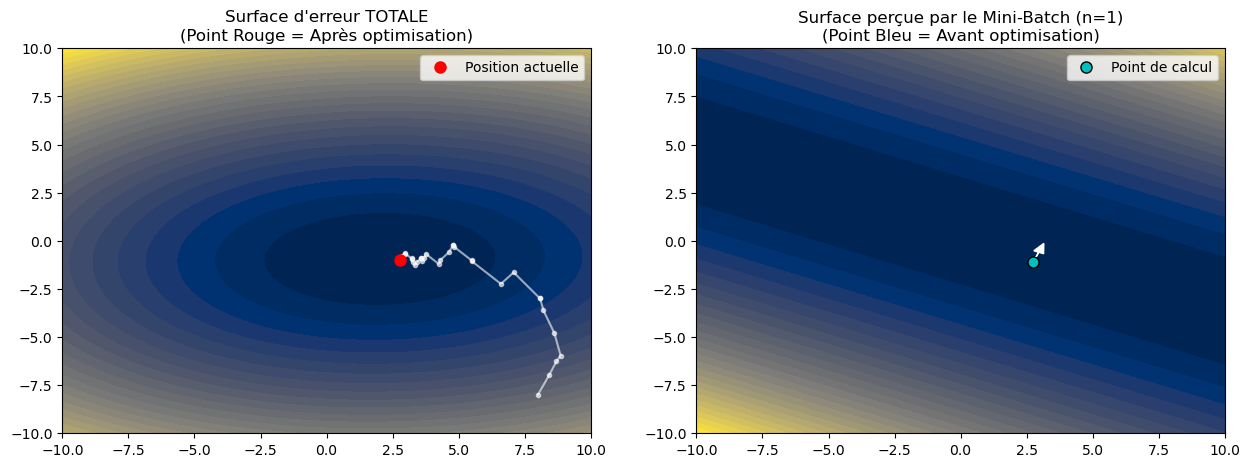
\includegraphics[height=0.35\linewidth]{Images/descente_gradient_stochastique}
		\label{fig:descente_gradient_stochastique}
		\caption*{Descente de gradient stochastique}
	\end{figure}
	Note: Les axes de la figure représentent les deux paramètres $W$ et $b$ d'un réseau de neurones: $\hat{Y} = X W + b$ avec $W \in \R$, $b \in \R$, $X \in \mathcal{M}_{n,1}(\R)$ et $\hat{Y} \in \mathcal{M}_{n,1}(\R)$.
\end{frame}

\begin{frame}{Descente de gradient stochastique, mini-batch, batch}
	\begin{figure}
		\centering
		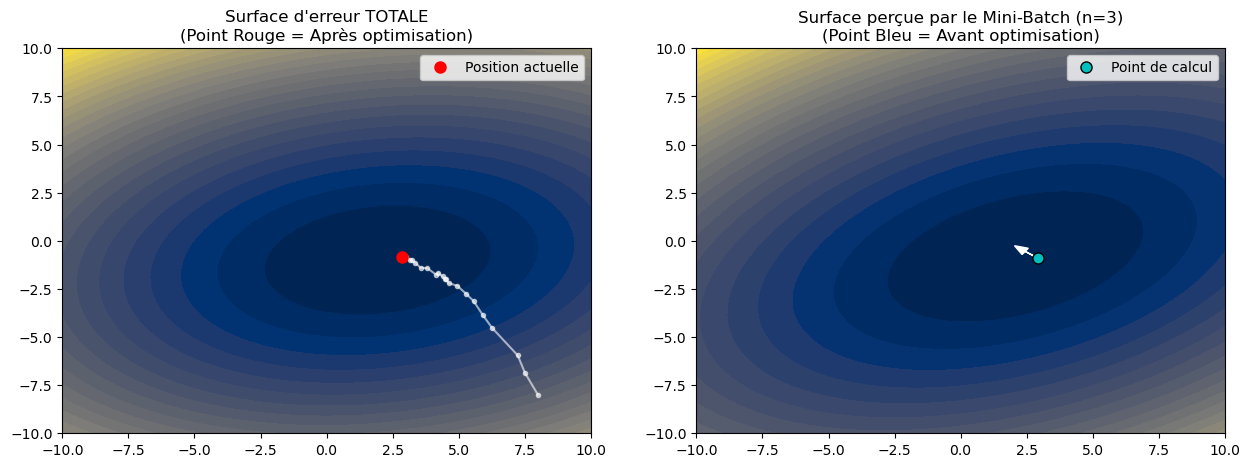
\includegraphics[height=0.35\linewidth]{Images/descente_gradient_minibatch}
		\label{fig:descente_gradient_mini_batch}
		\caption*{Descente de gradient en minibatch}
	\end{figure}
	Note: Les axes de la figure représentent les deux paramètres $W$ et $b$ d'un réseau de neurones: $\hat{Y} = X W + b$ avec $W \in \R$, $b \in \R$, $X \in \mathcal{M}_{n,1}(\R)$ et $\hat{Y} \in \mathcal{M}_{n,1}(\R)$.
\end{frame}

\begin{frame}{Descente de gradient stochastique, mini-batch, batch}
	\begin{figure}
		\centering
		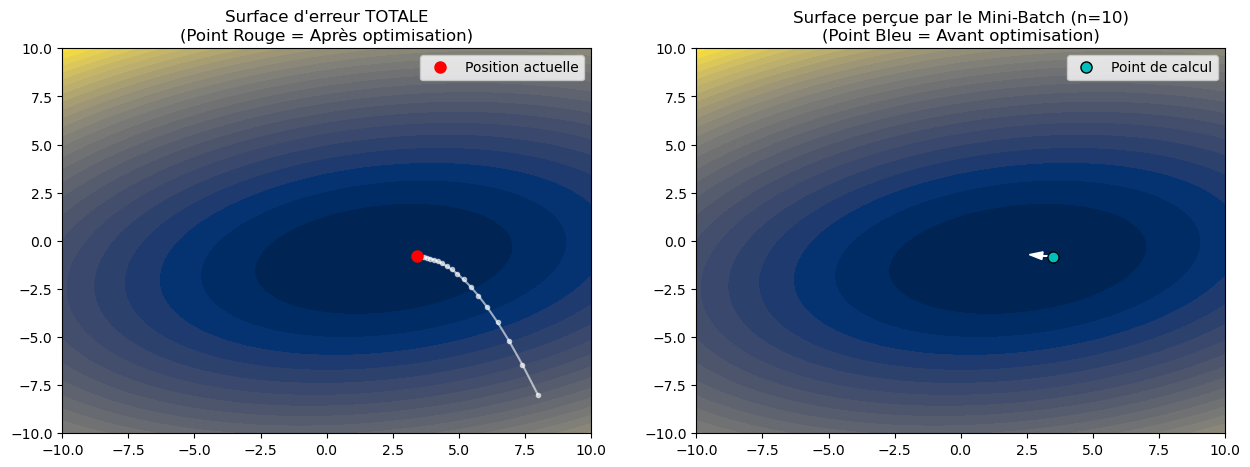
\includegraphics[height=0.35\linewidth]{Images/descente_gradient_batch}
		\label{fig:descente_gradient_batch}
		\caption*{Descente de gradient en batch}
	\end{figure}
	Note: Les axes de la figure représentent les deux paramètres $W$ et $b$ d'un réseau de neurones: $\hat{Y} = X W + b$ avec $W \in \R$, $b \in \R$, $X \in \mathcal{M}_{n,1}(\R)$ et $\hat{Y} \in \mathcal{M}_{n,1}(\R)$.
\end{frame}

\begin{frame}{Descente de gradient stochastique, mini-batch, batch}
	La forme de la fonction de coût en fonction des paramètres du réseau de neurones:
	\begin{itemize}
		\item est fixe !
		\pause
		\item ne dépend que de l'architecture du réseau (sa formulation mathématique) \textbf{et} des données d'entraînement.
		\pause
		\item est \textbf{inconnue} en général (dans les exemples ci-avant on a pu échantillonner facilement car il n'y a que 2 paramètres.)
		\pause
		\item n'est connue, après une passe avant qu'en un \textbf{seul point} ! La passe arrière nous permet de connaître le gradient en ce point.
	\end{itemize}
\end{frame}

\begin{frame}{Descente de gradient stochastique, mini-batch, batch}
	Si la passe avant n'est effectuée que sur un sous-ensemble des données d'apprentissage, tout se passe comme si on essayait d'optimiser une fonction de coût \textbf{différente}. La fonction vue par le mini-batch courant est l'image de droite sur les exemples ci-avant. C'est pour cela que:
	\begin{itemize}
		\item Le \textit{chemin} avec la descente de gradient stochastique est \textit{bruité}.
		\item Le \textit{chemin} avec la descente de gradient en mini-batch est moins \textit{bruité}, la fonction vue est une meilleure approximation de la vraie fonction de coût.
		\item Le \textit{chemin} avec la descente de gradient en batch est \textit{optimal}. Les gradients orientent l'optimiseur dans la \textbf{bonne} direction.
	\end{itemize}
\end{frame}

\begin{frame}{Descente de gradient stochastique, mini-batch, batch}
	\begin{itemize}
		\item Ce \textit{bruit} dans le parcours peut aider l'algorithme de descente gradient à mieux explorer l'espace des paramètres et à sortir de minima locaux. Ce type d'algorithme est en effet très sensible aux valeurs initiales mises dans les paramètres du réseau de neurones.
		\pause
		\item Mais ce chemin \textit{bruité} est aussi une perte de temps. Quand entraîner un réseau de neurones peut prendre des heures même sur un super-calculateur, tout gain de temps est appréciable !
	\end{itemize}
	
	\pause
	\vspace{0.5cm}
	
	Dans la suite de ce cours on explorera les techniques utilisées pour \textit{dé-bruiter} ce parcours même en utilisant des tailles de batchs petites en comparaison du nombre de données d'apprentissage.
	
\end{frame}

\subsection[Débruitage avec une moyenne par exponentielles pondérées]{Débruitage avec une moyenne par exponentielles pondérées}

\begin{frame}{Moyenne par exponentielles pondérées}
	Nous allons explorer une technique de \textit{dé-bruitage}: la \textbf{moyenne par exponentielles pondérées}:
	\begin{columns}
		\begin{column}{0.5\textwidth}
			\begin{figure}
				\centering
				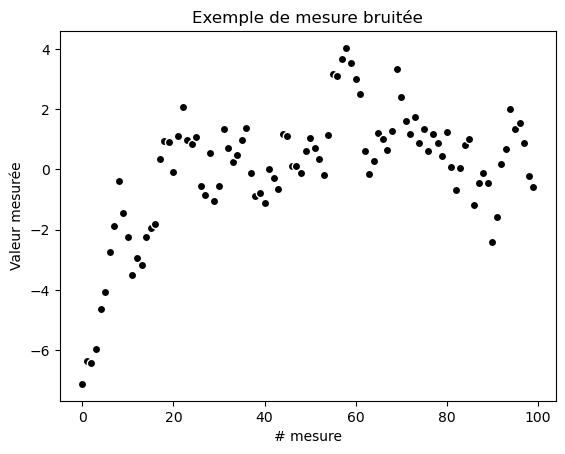
\includegraphics[width=1.0\linewidth]{Images/mesure_bruitee}
				\label{fig:mesure_bruitee}
			\end{figure}			
		\end{column}
		\begin{column}{0.5\textwidth}
			\begin{itemize}
				\item Soit une série de mesures effectuées.
				\item En traitement du signal, on dit en général qu'une \textbf{mesure} ou un \textbf{signal} est un mélange d'\textbf{information} (en général utile pour nos besoins !) et de \textbf{bruit}. 
				\item Plusieurs techniques existent pour \textit{dé-bruiter} ou \textit{lisser} un tel signal. On utilisera ici une moyenne par exponentielles pondérées.
			\end{itemize}
		\end{column}	
	\end{columns}
\end{frame}

\begin{frame}{Algorithme de la moyenne par exponentielles pondérées}
	On note $\theta$ la valeur de nos mesures. On les représentera par un vecteur dans $\R^n$ avec $n$ le nombre de mesures. $\theta_i$ est donc la i\textsuperscript{ème} mesure. On note $v \in \R$ une mesure dé-bruitée. On note enfin $\beta \in [0, 1]$ un coefficient de pondération. L'algorithme de la moyenne pondérée est le suivant:
	
	\begin{enumerate}
		\item On initialise $v = 0$.
		\item On fixe une valeur pour le coefficient de pondération $\beta$.
		\item Boucle sur les $n$ mesures:
		\begin{itemize}
			\item $\theta_i$ est la mesure courante.
			\item On calcule la mesure dé-bruitée $v \leftarrow (1 - \beta) \theta_i + \beta v$.
			\item On répète ce bloc jusqu'à ce que les $n$ mesures aient été traitées.
		\end{itemize}
	\end{enumerate}
\end{frame}

\begin{frame}{Algorithme de la moyenne par exponentielles pondérées}
	Le calcul de la mesure dé-bruitée implique donc une \textbf{moyenne} entre la mesure \textit{courante} et les mesures \textit{passées}:
	\begin{equation*}
		v^{(i)} = (1 - \beta) \theta_i + \beta v^{(i-1)}
	\end{equation*}
	En prenant $\beta = 0$, la mesure dé-bruitée est en fait la mesure elle-même, sans dé-bruitage, $\theta_i$. Une valeur de $\beta = 1$ résulterait en un signal dé-bruité constant et égal à 0 puisque $v$ est initialisée à 0.
	
	\pause
	\vspace{0.5cm}
	
	En prenant $\beta = 0.9$, on peut regarder ce qu'il se passe sur la 3\textsuperscript{ème} mesure:
	\begin{equation*}
		\begin{aligned}
			v^{(3)} 
			&= (1 - \beta) \theta_3 + \beta v^{(2)} \\
			&= (1 - \beta) \theta_3 + \beta \left((1 - \beta) \theta_{2} + \beta v^{(1)} \right) \\
			&= (1 - \beta) \theta_3 + \beta (1 - \beta) \theta_{2} + \beta^2 v^{(1)} \\
			&= (1 - \beta) \theta_3 + \beta (1 - \beta) \theta_{2} + \beta^2 (1 - \beta) \theta_{1} + \underbrace{\beta^3 v^{(0)}}_{= 0}
		\end{aligned}
	\end{equation*}
\end{frame}

\begin{frame}{Algorithme de la moyenne par exponentielles pondérées}
	On peut maintenant réaliser l'application numérique:
	\begin{equation*}
		\begin{aligned}
			v^{(3)} 
			&= (1 - \beta) \theta_3 + \beta (1 - \beta) \theta_{2} + \beta^2 (1 - \beta) \theta_{1} \\
			&= (1 - 0.9) \theta_3 + 0.9 (1 - 0.9) \theta_{2} + 0.9^2 (1 - 0.9) \theta_{1} \\
			&= 0.1 \cdot \theta_3 + 0.09 \cdot \theta_{2} + 0.081 \cdot \theta_{1}
		\end{aligned}
	\end{equation*}
	On voit donc que la pondération associée à chaque mesure décroit au fur et à mesure que l'on s'\textit{éloigne} de la mesure courante.
\end{frame}

\begin{frame}{Moyenne par exponentielles pondérées}
	\begin{columns}
		\begin{column}{0.5\textwidth}
			\begin{figure}
				\centering
				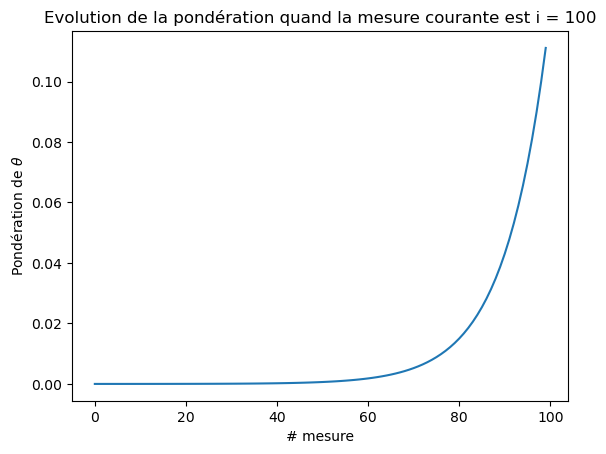
\includegraphics[width=1.0\linewidth]{Images/mep_decroissance}
				\label{fig:mep_decroissance}
			\end{figure}			
		\end{column}
		\begin{column}{0.5\textwidth}
			Ce tracé graphique illustre la décroissance de la pondération pour chaque mesure lorsque la mesure courante est la 100\textsuperscript{ème}. On voit clairement la fonction puissance de $\beta$ qui donne son qualificatif d'\textbf{exponentielle} à la méthode !
		\end{column}	
	\end{columns}
\end{frame}

\begin{frame}{Moyenne par exponentielles pondérées}
	\begin{columns}
		\begin{column}{0.5\textwidth}
			\begin{figure}
				\centering
				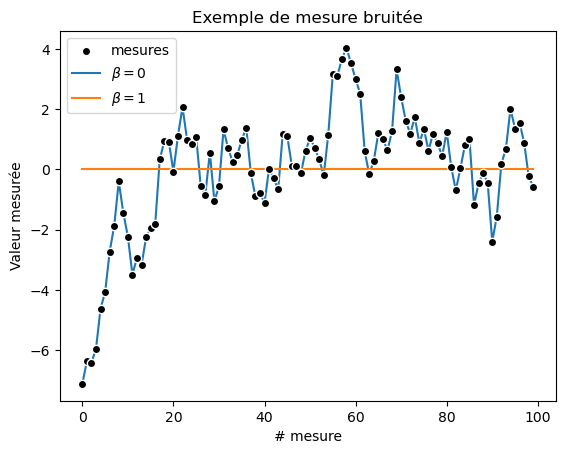
\includegraphics[width=1.0\linewidth]{Images/mesure_bruitee_extremes}
				\label{fig:mesure_bruitee_extremes}
			\end{figure}			
		\end{column}
		\begin{column}{0.5\textwidth}
			\begin{figure}
				\centering
				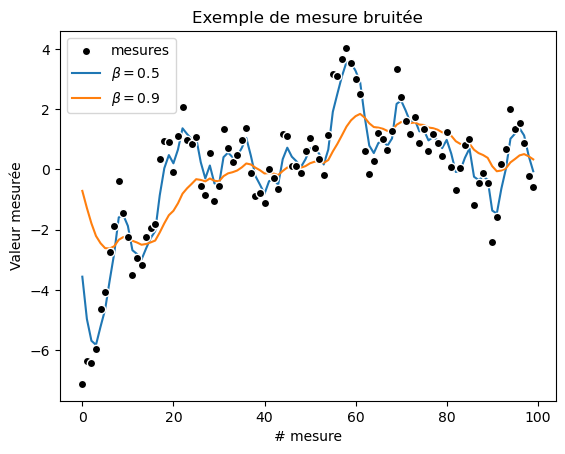
\includegraphics[width=1.0\linewidth]{Images/mesure_bruitee_raisonnable}
				\label{fig:mesure_bruitee_raisonnable}
			\end{figure}			
		\end{column}	
	\end{columns}
	\pause
	On voit bien l'influence du $\beta$ sur le lissage: plus $\beta$ augmente, plus le lissage est important. Mais n'y a-t-il pas un problème pour les toutes premières mesures ?
\end{frame}

\begin{frame}{Algorithme de la moyenne par exponentielles pondérées}
	Le problème au démarrage est lié à l'initialisation de $v = 0$. Pour la première mesure on a donc:
	\begin{equation*}
		v^{(1)} = (1 - \beta) \theta_1 + \beta v^{(0)} = (1 - \beta) \theta_1
	\end{equation*}
	Donc plus $\beta$ est grand, et plus la première mesure dé-bruitée est \textit{tirée} vers 0. Pour corriger ce problème on introduit une \textbf{correction de biais}:
	\pause
	\begin{equation*}
		\begin{cases}
			v^{(i)} = (1 - \beta) \theta_i + \beta v^{(i-1)} \\
			\hat{v}^{(i)} = \displaystyle \frac{v^{(i)}}{1 - \beta^i}
		\end{cases}
	\end{equation*}
	\pause
	Pour la première mesure $i = 1$, cela revient donc à calculer: $\hat{v}^{(1)} = \theta_1$. Ce qui \textit{corrige complètement} le dé-bruitage. Plus $i$ augmente, et plus le facteur de correction tend vers 1, il n'a donc pas d'influence pour les mesures \textit{éloignées} de la première.
	
	\vspace{0.2cm}
	
	\textbf{Attention}: dans l'implémentation de l'algorithme, la mise à jour de $v$ se fait à partir du $v$ précédent et pas du $\hat{v}$ précédent.
\end{frame}

\begin{frame}{Algorithme de la moyenne par exponentielles pondérées}
	Voici l'algorithme introduisant la correction de biais:
	\begin{enumerate}
		\item On initialise $v = 0$.
		\item On fixe une valeur pour le coefficient de pondération $\beta$.
		\item Boucle sur les $n$ mesures:
		\begin{itemize}
			\item $\theta_i$ est la mesure courante.
			\item On calcule la mesure dé-bruitée $v \leftarrow (1 - \beta) \theta_i + \beta v$.
			\item On applique la correction de biais: $\hat{v} \leftarrow \frac{v}{1 - \beta^i}$
		\end{itemize}
	\end{enumerate}
\end{frame}

\begin{frame}{Moyenne par exponentielles pondérées}
	Les tracés ci-dessous montrent l'influence de la correction de biais pour deux valeurs différentes de $\beta$:
	\begin{columns}
		\begin{column}{0.5\textwidth}
			\begin{figure}
				\centering
				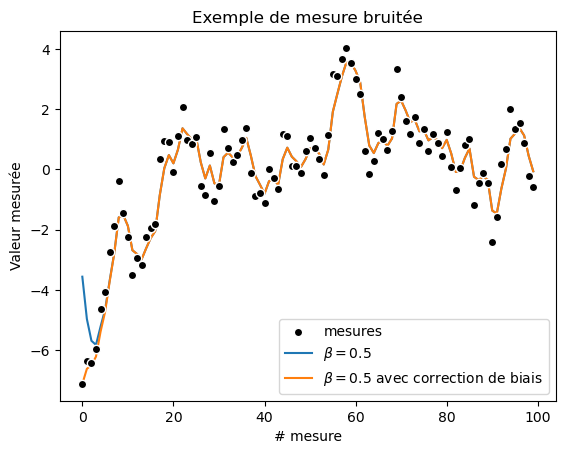
\includegraphics[width=1.0\linewidth]{Images/mesure_bruitee_biais1}
				\label{fig:mesure_bruitee_biais1}
			\end{figure}			
		\end{column}
		\begin{column}{0.5\textwidth}
			\begin{figure}
				\centering
				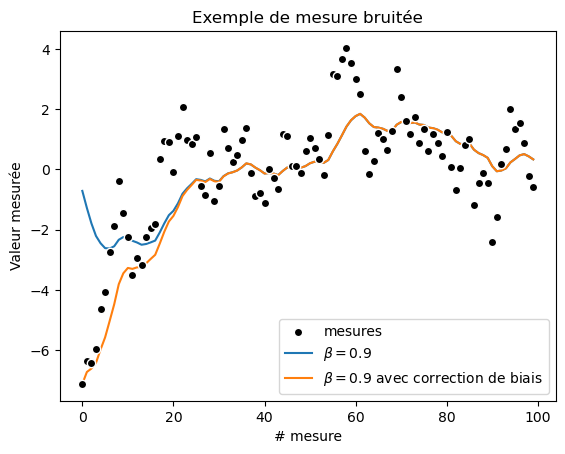
\includegraphics[width=1.0\linewidth]{Images/mesure_bruitee_biais2}
				\label{fig:mesure_bruitee_biais2}
			\end{figure}			
		\end{column}	
	\end{columns}
\end{frame}

\begin{frame}{Moyenne par exponentielles pondérées}
	Cet algorithme est certes \textbf{rudimentaire} mais extrêmement efficace pour les applications en apprentissage automatique:
	\begin{itemize}
		\item Il est \textbf{rapide}: le dé-bruitage est simple et se fait en deux étapes si on effectue une correction de biais.
		\item Il est sobre en \textbf{mémoire}: il y a une simple \textit{valeur} à stocker en mémoire.
	\end{itemize}
	Cet algorithme est alors implémenté pour \textbf{améliorer} les algorithmes de descente de gradient:
	\begin{itemize}
		\item En dé-bruitant la \textbf{\textit{trajectoire}} des paramètres (premier moment): méthode du \textbf{momentum}.
		\item En adaptant le pas en fonction des \textbf{\textit{oscillations}} (second moment): algorithme de \textbf{RMSprop}.
		\item En combinant trajectoire et pas adaptatif: algorithme de \textbf{Adam}.
	\end{itemize}
\end{frame}

\subsection[Descente de gradient avec momentum]{Descente de gradient avec momentum}

\begin{frame}{Descente de gradient avec momentum}
	L'algorithme de la descente du gradient avec momentum, développée par Boris Polyak en 1964, \textit{dé-bruite} la trajectoire des paramètres en utilisant l'algorithme de lissage des moyennes par pondération exponentielle qu'il applique sur le \textbf{gradient}. On notera $\beta_1$ le coefficient de pondération dans ce lissage:
	\begin{enumerate}
		\item Les paramètres $P$ sont initialisés.
		\pause
		\item Pour chaque paramètre on initialise $v_P = 0$.
		\pause
		\item Boucle sur les époques.
		\pause
		\item Pour chaque batch de taille $m$:
		\begin{itemize}
			\item Calcul de la passe avant et de l'erreur $e$.
			\pause
			\item Application de la rétro-propagation du gradient pour calculer $\nabla_P = \frac{\partial{e}}{\partial{P}}$ pour tous les paramètres $P$.
			\pause
			\item Calcul du lissage du gradient: $v_P \leftarrow (1 - \beta_1) \nabla_P + \beta_1 v_P$
			\pause 
			\item Mise à jour de chaque paramètre $P \leftarrow P - \alpha v_P$
		\end{itemize}
		\item Retour à l'étape 3 tant qu'un critère d'arrêt n'est pas rencontré.
	\end{enumerate}	
\end{frame}

\begin{frame}{Visualisation - Descente de gradient avec momentum}
	Résultat d'une descente de gradient avec momentum ($\beta_1 = 0.9$) pour une taille de mini-batch $m = 1$ et $\alpha = 0.1$:
	\begin{figure}
		\centering
		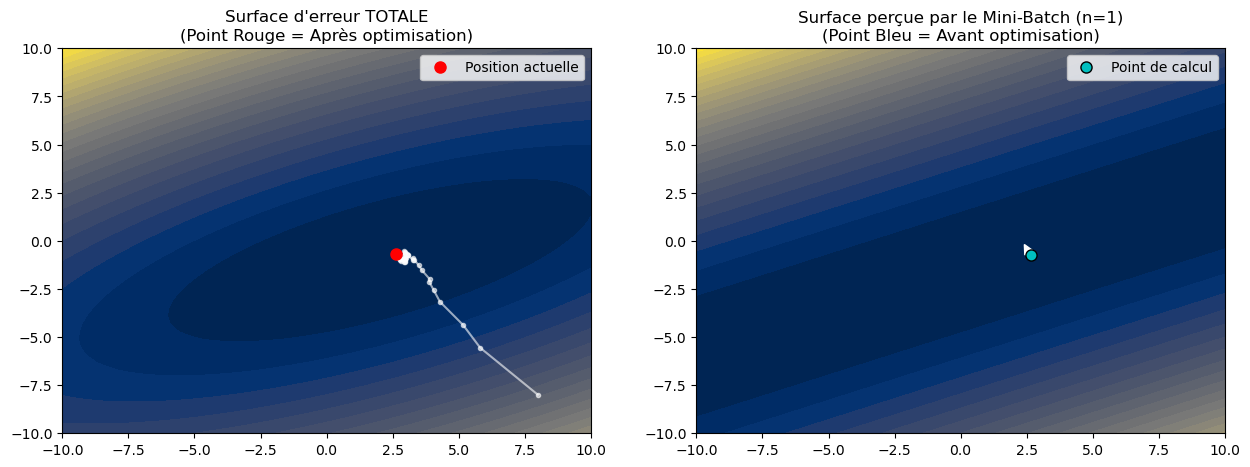
\includegraphics[height=0.35\linewidth]{Images/descente_gradient_momentum}
		\label{fig:descente_gradient_momentum}
	\end{figure}
	Note: Les axes de la figure représentent les deux paramètres $W$ et $b$ d'un réseau de neurones: $\hat{Y} = X W + b$ avec $W \in \R$, $b \in \R$, $X \in \mathcal{M}_{n,1}(\R)$ et $\hat{Y} \in \mathcal{M}_{n,1}(\R)$.
\end{frame}

\subsection[Algorithme RMSprop]{Algorithme RMSprop}

\begin{frame}{Algorithme RMSprop}
	L'algorithme RMSprop (RMS pour root mean square) utilise un lissage du \textbf{carré des gradients} et propose, dans la mise à jour des paramètres, de \textbf{diviser} le terme $\alpha \nabla_P$ par la racine carrée de l'historique de ses carrés lissés. Cela revient en fait à \textbf{adapter} le taux d'apprentissage:
	\begin{itemize}
		\item Dans les zones de \textbf{fort gradients}, les pas sont réduits afin de garantir une stabilité numérique à la descente de gradient: la vitesse \textbf{ralentit}.
		\item Dans les zones de \textbf{faibles gradients}, les pas sont augmentés afin d'accélérer la convergence: la vitesse \textbf{augmente}.
	\end{itemize}
	Le momentum permet de gagner du temps dans l'optimisation parce qu'il lisse la trajectoire et RMSprop permet de gagner du temps parce qu'il nous permet de travailler avec un taux d'apprentissage plus fort tout en gardant une optimisation numériquement stable.
	
	\vspace{0.3cm}
	
	L'algorithme a été introduit par Geoffrey Hinton dans un de ses cours en ligne en 2012. Il est un des pères fondateur de l'apprentissage profond et l'auteur de l'article sur la rétro-propagation du gradient.
\end{frame}

\begin{frame}{Algorithme RMSprop}
	On notera $\beta_2$ le coefficient de pondération dans ce lissage des gradients au carré. $\epsilon$ représente un nombre réel très petit (typiquement $10^{-8}$) pour éviter une division par zéro:
	\begin{enumerate}
		\item Les paramètres $P$ sont initialisés.
		\pause
		\item Pour chaque paramètre on initialise $s_P = 0$.
		\pause
		\item Boucle sur les époques.
		\pause
		\item Pour chaque batch de taille $m$:
		\begin{itemize}
			\item Calcul de la passe avant et de l'erreur $e$.
			\pause
			\item Application de la rétro-propagation du gradient pour calculer $\nabla_P = \frac{\partial{e}}{\partial{P}}$ pour tous les paramètres $P$.
			\pause
			\item Lissage du carré du gradient: $s_P \leftarrow (1 - \beta_2) \nabla_P^2 + \beta_2 s_P$
			\pause 
			\item Mise à jour de chaque paramètre $P \leftarrow P - \frac{\alpha}{\sqrt{s_P} + \epsilon} \nabla_P$
		\end{itemize}
		\item Retour à l'étape 3 tant qu'un critère d'arrêt n'est pas rencontré.
	\end{enumerate}	
\end{frame}

\begin{frame}{Visualisation - Algorithme RMSprop}
	Résultat de l'algorithme RMSprop ($\beta_2 = 0.99$) pour une taille de mini-batch $m = 1$ et $\alpha = 0.2$:
	\begin{figure}
		\centering
		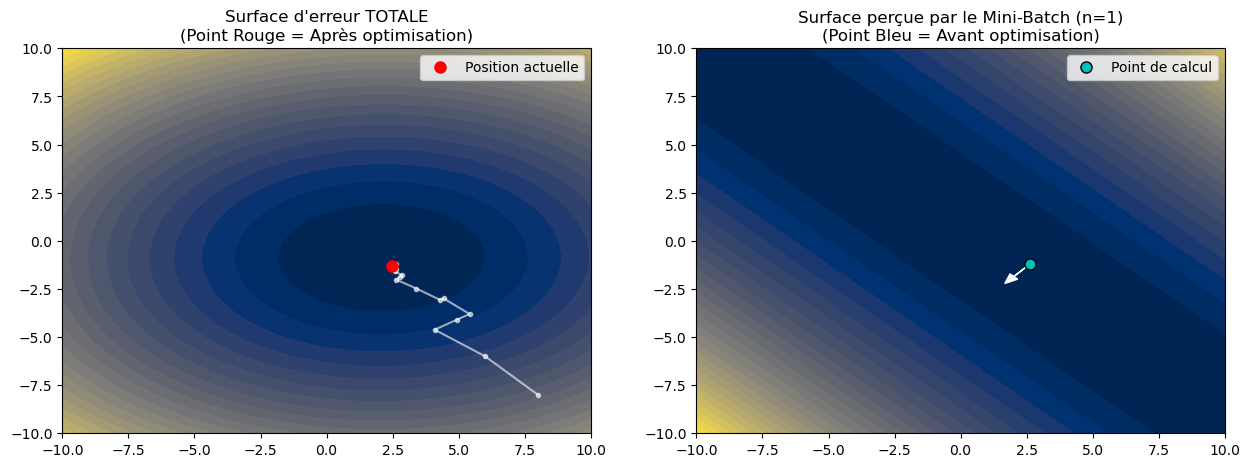
\includegraphics[height=0.35\linewidth]{Images/descente_gradient_rmsprop}
		\label{fig:descente_gradient_prop}
	\end{figure}
	Note: Les axes de la figure représentent les deux paramètres $W$ et $b$ d'un réseau de neurones: $\hat{Y} = X W + b$ avec $W \in \R$, $b \in \R$, $X \in \mathcal{M}_{n,1}(\R)$ et $\hat{Y} \in \mathcal{M}_{n,1}(\R)$.
\end{frame}

\subsection[Algorithme Adam]{Algorithme Adam}

\begin{frame}{Algorithme Adam}
	L'algorithme Adam (ADAptive Moment estimation) est une \textbf{combinaison} d'un descente de gradient avec momentum ($\beta_1$) et une adaptation du taux d'apprentissage avec de RMSprop ($\beta_2$) incluant des \textbf{corrections de biais}.
	
	\vspace{0.5cm}
	
	Il a été développé en 2014 par Diederik Kingma et Jimmy Ba et l'article est l'un des plus cités de toute l'histoire de l'informatique et de l'intelligence artificielle.
		
\end{frame}

\begin{frame}{Algorithme Adam}
	L'algorithme Adam peut être décrit comme suit:
	\begin{enumerate}
		\item Les paramètres $P$ sont initialisés.
		\pause
		\item On initialise un compteur d'itérations $t = 0$.
		\pause
		\item Pour chaque paramètre on initialise $v_P = 0$ et $s_P = 0$.
		\pause
		\item Boucle sur les époques.
		\pause
		\item Pour chaque batch de taille $m$:
		\begin{itemize}
			\item Mise à jour du numéro d'itération $t \leftarrow t + 1$.
			\pause
			\item Calcul de la passe avant et de l'erreur $e$.
			\pause
			\item Calcul de $\nabla_P = \frac{\partial{e}}{\partial{P}}$ pour tous les paramètres $P$.
			\pause
			\item Lissage du gradient: $v_P \leftarrow (1 - \beta_1) \nabla_P + \beta_1 v_P$
			\pause 
			\item Lissage du carré du gradient: $s_P \leftarrow (1 - \beta_2) \nabla_P^2 + \beta_2 s_P$
			\pause
			\item Corrections de biais: $\widehat{v_P} = v_P / (1 - \beta_1^t)$ et $\widehat{s_P} = s_P / (1 - \beta_2^t)$
			\item Mise à jour de chaque paramètre: $P \leftarrow P - \frac{\alpha}{\sqrt{\widehat{s_P}} + \epsilon} \widehat{v_P}$
		\end{itemize}
		\item Retour à l'étape 4 tant qu'un critère d'arrêt n'est pas rencontré.		
	\end{enumerate}	
\end{frame}

\begin{frame}{Visualisation - Algorithme Adam}
	Résultat de l'algorithme Adam ($\beta_1 = 0.9$ et $\beta_2 = 0.99$) pour une taille de mini-batch $m = 1$ et $\alpha = 0.3$:
	\begin{figure}
		\centering
		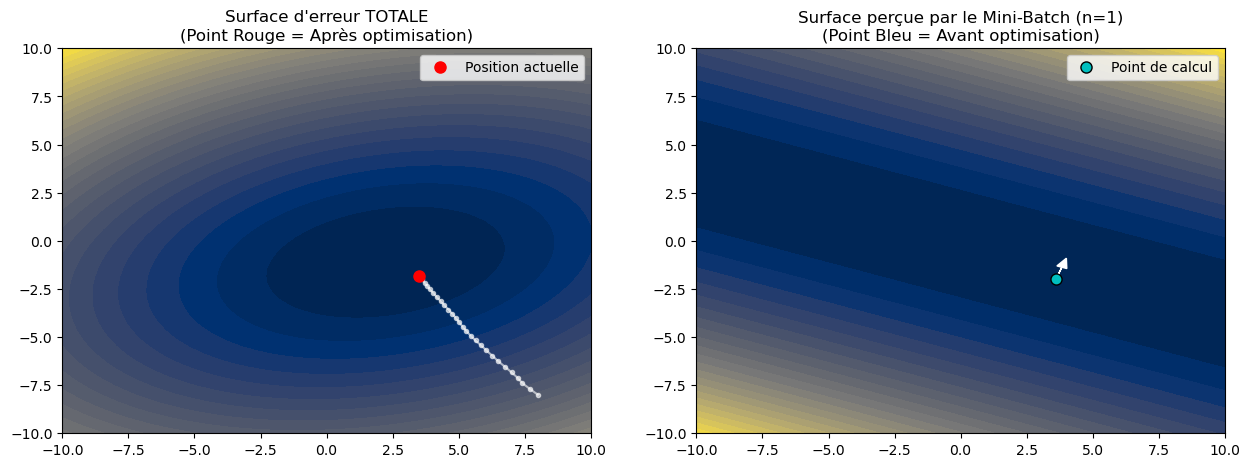
\includegraphics[height=0.35\linewidth]{Images/descente_gradient_adam}
		\label{fig:descente_gradient_adam}
	\end{figure}
	Note: Les axes de la figure représentent les deux paramètres $W$ et $b$ d'un réseau de neurones: $\hat{Y} = X W + b$ avec $W \in \R$, $b \in \R$, $X \in \mathcal{M}_{n,1}(\R)$ et $\hat{Y} \in \mathcal{M}_{n,1}(\R)$.
\end{frame}

\subsection[Conclusions pour l'optimisation]{Conclusions pour l'optimisation}

\begin{frame}{Conclusions}
	Nous avons vu trois algorithmes différents pour l'optimisation des paramètres dans un réseau de neurones. \textbf{Adam} implémente deux méthodes permettant d'optimiser ses performances et ce pour une variété de réseaux de neurones qui dépasse le cadre de ce cours. Il s'est donc imposé comme l'algorithme \textbf{standard} d'\textbf{optimisation} pour les réseaux de neurones, même pour les réseaux profonds.
	
	\pause
	\vspace{0.5cm}
	
	Nous avons aussi discuté de l'hyper-paramètre \textbf{taille de batch} $m$, qui établit un compromis entre le fait de tirer bénéfice au maximum de la capacité de vectorisation des ordinateurs sans trop surcharger la mémoire. La taille de batch influe également sur la \textit{trajectoire} d'optimisation, même si la méthode du momentum tend à la lisser.
\end{frame}

\subsection[Initialisation des poids et disparition du gradient]{Initialisation des poids et disparition du gradient}

\begin{frame}{Le problème de la disparition et de l'explosion du gradient}
	Jusqu'ici, nous avons simplement dit: on initialise \textit{aléatoirement} les paramètres du réseau de neurones. Dans cette section, nous discuterons  \textit{comment} procéder à cette initialisation. Dans les réseaux de neurones, encore plus quand ils sont profonds, deux phénomènes peuvent survenir qui mettent à mal la rétro-propagation du gradient:
	\begin{itemize}
		\item \textbf{L'explosion du gradient} : Si les poids sont initialisés avec des valeurs trop grandes, le gradient est multiplié par des valeurs supérieures à 1 à chaque couche. Il grandit de manière exponentielle jusqu'à ne plus pouvoir être représenté correctement par l'ordinateur (overflow numérique).
		\pause
		\item \textbf{La disparition du gradient} (\textit{vanishing gradient}) : Si les poids sont trop petits, ou si les fonctions d'activation saturent, le gradient est multiplié par des valeurs proches de 0 à chaque couche. Il s'éteint avant d'atteindre les premières couches. Si les gradients sont nuls dans les premières couches alors ils ne sont jamais mis à jour par l'algorithme d'optimisation.
	\end{itemize}
\end{frame}

\begin{frame}{Logique mathématique: préserver la variance}
	La solution consiste à contrôler rigoureusement la \textbf{variance} des activations et des gradients à travers les couches grâce à une initialisation intelligente des poids.
	
	\pause
	\vspace{0.2cm}
	
	Considérons une couche linéaire sans biais $Z = X W$ où $X \in \mathcal{M}_{n, u}(\R)$, $W \in \mathcal{M}_{u, v}(\R)$ et $Z \in \mathcal{M}_{n, u}(\R)$. On cherche à ce que la variance de la sortie $Z$ soit égale à la variance de l'entrée $X$ pour éviter que le signal ne s'éteigne ou n'explose.
	
	\pause
	\vspace{0.2cm}
	
	En supposant les entrées et les poids indépendants (leur covariance est nulle), centrés ($\E{X}=0, \E{W}=0$) et de même loi, on peut montrer que:
	\begin{equation*}
		\Var{Z^{(i)}_j} = u \cdot \Var{X^{(i)}_k} \cdot \Var{W_{k,j}}
	\end{equation*}
		
	\pause
	\vspace{0.2cm}
	
	Pour obtenir $\Var{Z^{(i)}_j} = \Var{X^{(i)}_k}$, il faut impérativement que :
	\begin{equation*}
		\Var{W_{k,j}} = \frac{1}{u}
	\end{equation*}
\end{frame}

\begin{frame}{Initialisation de Xavier / Glorot (Logistique et Tanh)}
	Pour la fonction logistique, Xavier Glorot et Yoshua Bengio (2010) ont proposé de moyenner les contraintes de la passe avant ($n_{\text{in}}$) et de la passe arrière ($n_{\text{out}}$):
	
	\begin{block}{Initialisation de Xavier (Fonction logistique)}
		Pour une couche ayant $n_{\text{in}}$ entrées et $n_{\text{out}}$ sorties, on initialise les poids selon une loi normale centrée :
		\begin{equation*}
			W_{i,j} \sim \mathcal{N}\left(0, \, \sigma^2\right) \quad \text{avec} \quad \sigma = \sqrt{\frac{2}{n_{\text{in}} + n_{\text{out}}}}
		\end{equation*}
		Ou selon une loi uniforme:
		\begin{equation*}
			W_{i,j} \sim \mathcal{U}\left(-\sqrt{\frac{6}{n_{\text{in}} + n_{\text{out}}}}, \, \sqrt{\frac{6}{n_{\text{in}} + n_{\text{out}}}}\right)
		\end{equation*}
		Les deux lois disposent de la même variance $\frac{2}{n_{\text{in}} + n_{\text{out}}}$.
	\end{block}
\end{frame}

\begin{frame}{Visualisation - Xavier pour la fonction logistique}
	\begin{columns}
		\begin{column}{0.65\textwidth}
			\begin{figure}
				\centering
				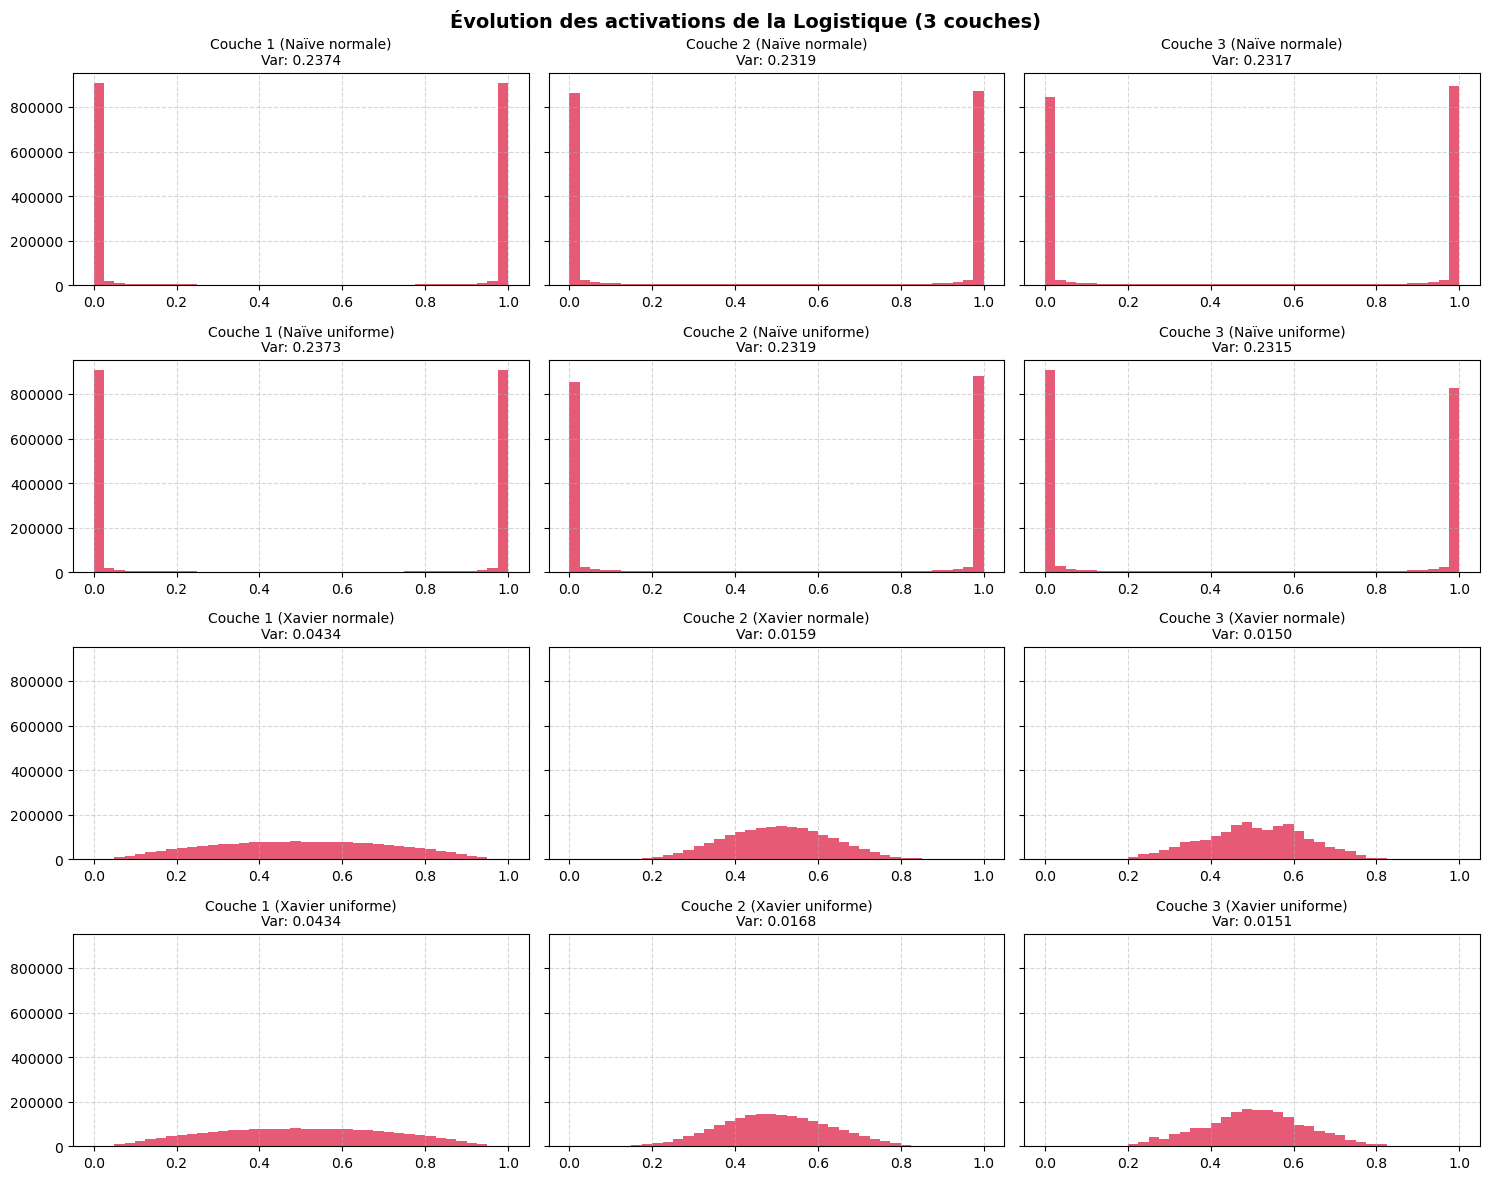
\includegraphics[width=1.0\linewidth]{Images/xavier_logistique}
				\label{fig:xavier_logistique}
			\end{figure}				
		\end{column}
		\begin{column}{0.35\textwidth}
			Avec une initialisation naïve des poids centrés en 0 et de variance unitaire, on sature la fonction logistique très rapidement. Les gradients sont nuls, le réseau n'apprend pas.
			
			\vspace{0.5cm}
			
			Même si on ne sature pas avec l'initialisation de Xavier, on observe une chute rapide de la variance. C'est pour cela que l'on n'utilise plus la fonction logistique dans les couches cachées.
		\end{column}
	\end{columns}
\end{frame}

\begin{frame}{Initialisation de Xavier / Glorot (Logistique et Tanh)}
	Pour la fonction tangente hyperbolique, un terme de gain $\gamma = \frac{5}{3}$, il vient corriger l'effet de la non-linéarité sur la variance:
	
	\begin{block}{Initialisation de Xavier (Fonction tangente hyperbolique)}
		Pour une couche ayant $n_{\text{in}}$ entrées et $n_{\text{out}}$ sorties, on initialise les poids selon une loi normale centrée :
		\begin{equation*}
			W_{i,j} \sim \mathcal{N}\left(0, \, \sigma^2\right) \quad \text{avec} \quad \sigma = \gamma  \sqrt{\frac{2}{n_{\text{in}} + n_{\text{out}}}}
		\end{equation*}
		Ou selon une loi uniforme:
		\begin{equation*}
			W_{i,j} \sim \mathcal{U}\left(-\gamma \sqrt{\frac{6}{n_{\text{in}} + n_{\text{out}}}}, \,  \gamma \sqrt{\frac{6}{n_{\text{in}} + n_{\text{out}}}}\right)
		\end{equation*}
		Les deux lois disposent de la même variance $\frac{2 \gamma^2}{n_{\text{in}} + n_{\text{out}}}$.
	\end{block}
\end{frame}

\begin{frame}{Visualisation - Xavier pour la fonction tangente hyperbolique}
	\begin{columns}
		\begin{column}{0.65\textwidth}
			\begin{figure}
				\centering
				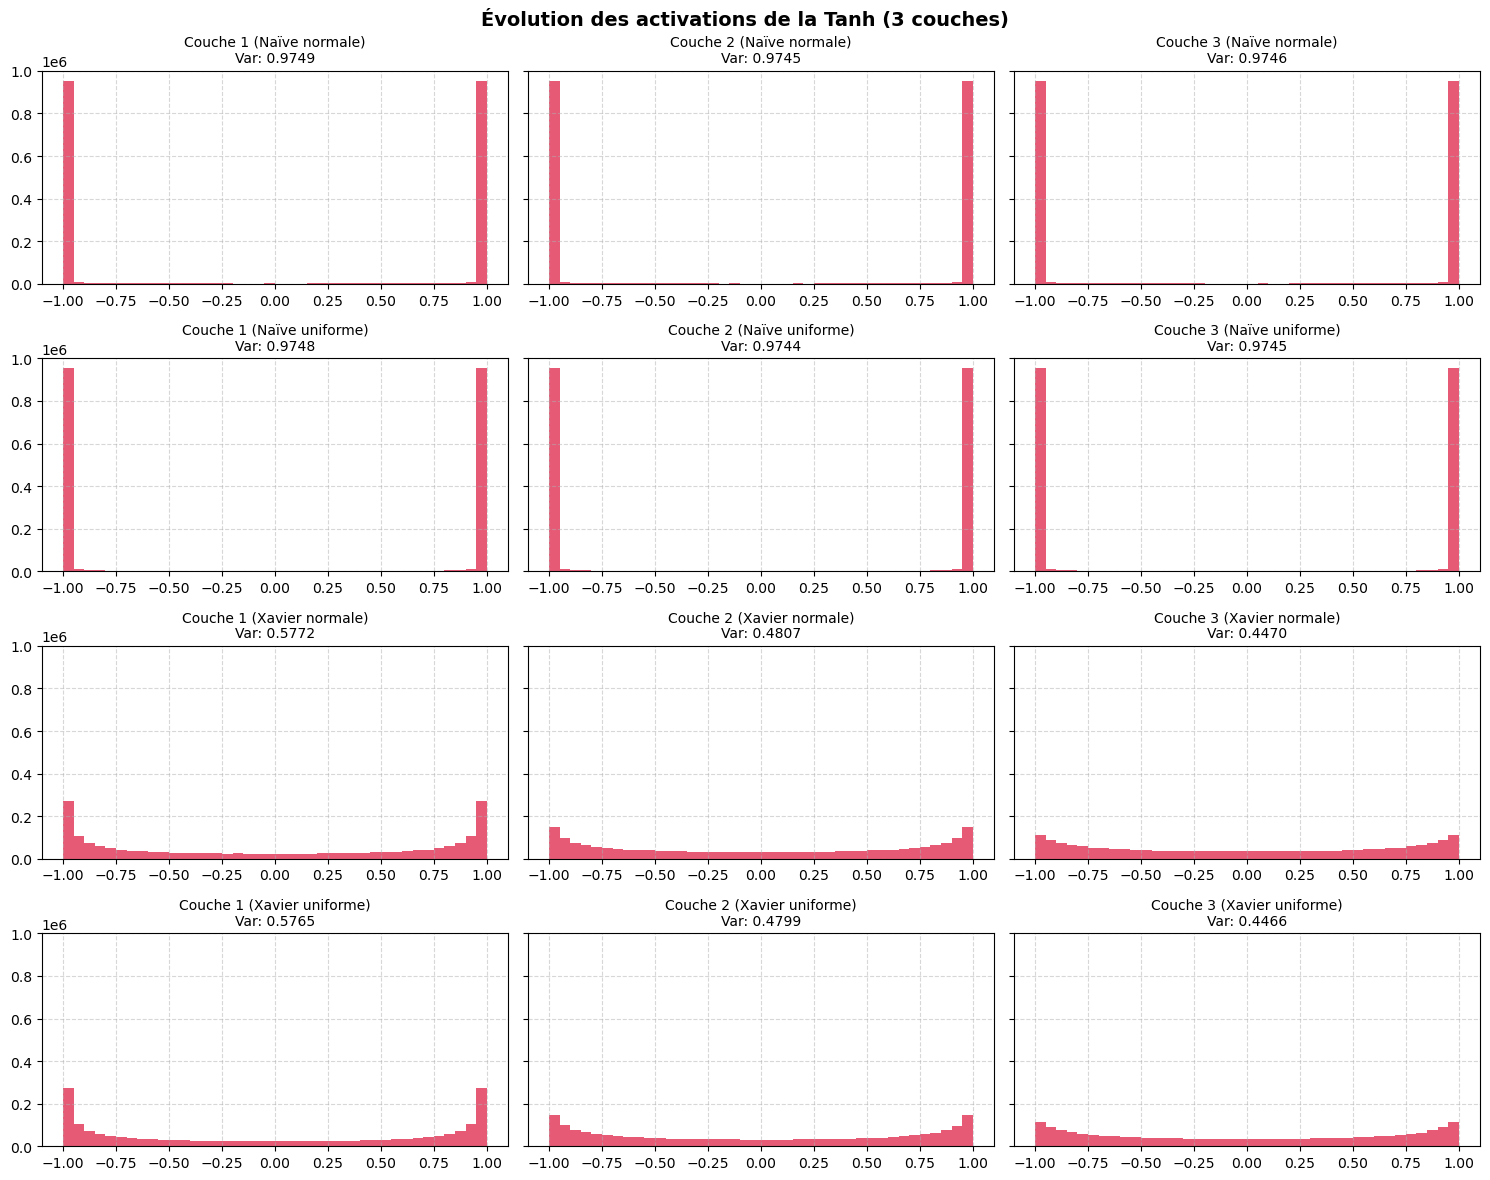
\includegraphics[width=1.0\linewidth]{Images/xavier_tanh}
				\label{fig:xavier_tanh}
			\end{figure}				
		\end{column}
		\begin{column}{0.35\textwidth}
			Avec une initialisation naïve des poids centrés en 0 et de variance unitaire, on observe la même saturation.
			
			\vspace{0.5cm}
			
			Avec l'intialisation de Xavier (uniforme ou normale) nous n'observons ni saturation excessive ni effondrement de la variance !
		\end{column}
	\end{columns}
\end{frame}

\begin{frame}{Initialisation de Kaiming / He (ReLU)}
	La fonction $\operatorname{ReLU}(Z) = \max(0, Z)$ brise l'hypothèse de symétrie : elle met à zéro exactement la moitié de ses entrées en moyenne. Le signal perd la moitié de sa variance à chaque passage ! 
	
	\pause
	\vspace{0.5cm}
	
	Pour compenser cette perte de variance, Kaiming He (2015) a démontré qu'il fallait doubler la variance des poids initiaux. L'article ne mentionnait qu'une initialisation utilisant une loi normale, mais la communauté a rapidement proposé une alternative basée sur une loi uniforme de même variance.
\end{frame}

\begin{frame}{Initialisation de Kaiming / He (ReLU)}
	
	\begin{block}{Initialisation de Kaiming (Fonction ReLU)}
		Pour une couche d'activation ReLU ayant $n_{\text{in}}$ entrées, on initialise les poids selon une loi normale centrée :
		\begin{equation*}
			W_{i,j} \sim \mathcal{N}\left(0, \, \sigma^2\right) \quad \text{avec} \quad \sigma = \sqrt{\frac{2}{n_{\text{in}}}}
		\end{equation*}	
		Ou selon une loi uniforme:
		\begin{equation*}
			W_{i,j} \sim \mathcal{U}\left(-\sqrt{\frac{6}{n_{\text{in}}}}, \, \sqrt{\frac{6}{n_{\text{in}}}}\right)
		\end{equation*}
		Les deux lois disposent de la même variance $\frac{2}{n_{\text{in}}}$.
	\end{block}
	
\end{frame}

\begin{frame}{Visualisation - Kaiming pour la fonction ReLU}
	\begin{columns}
		\begin{column}{0.65\textwidth}
			\begin{figure}
				\centering
				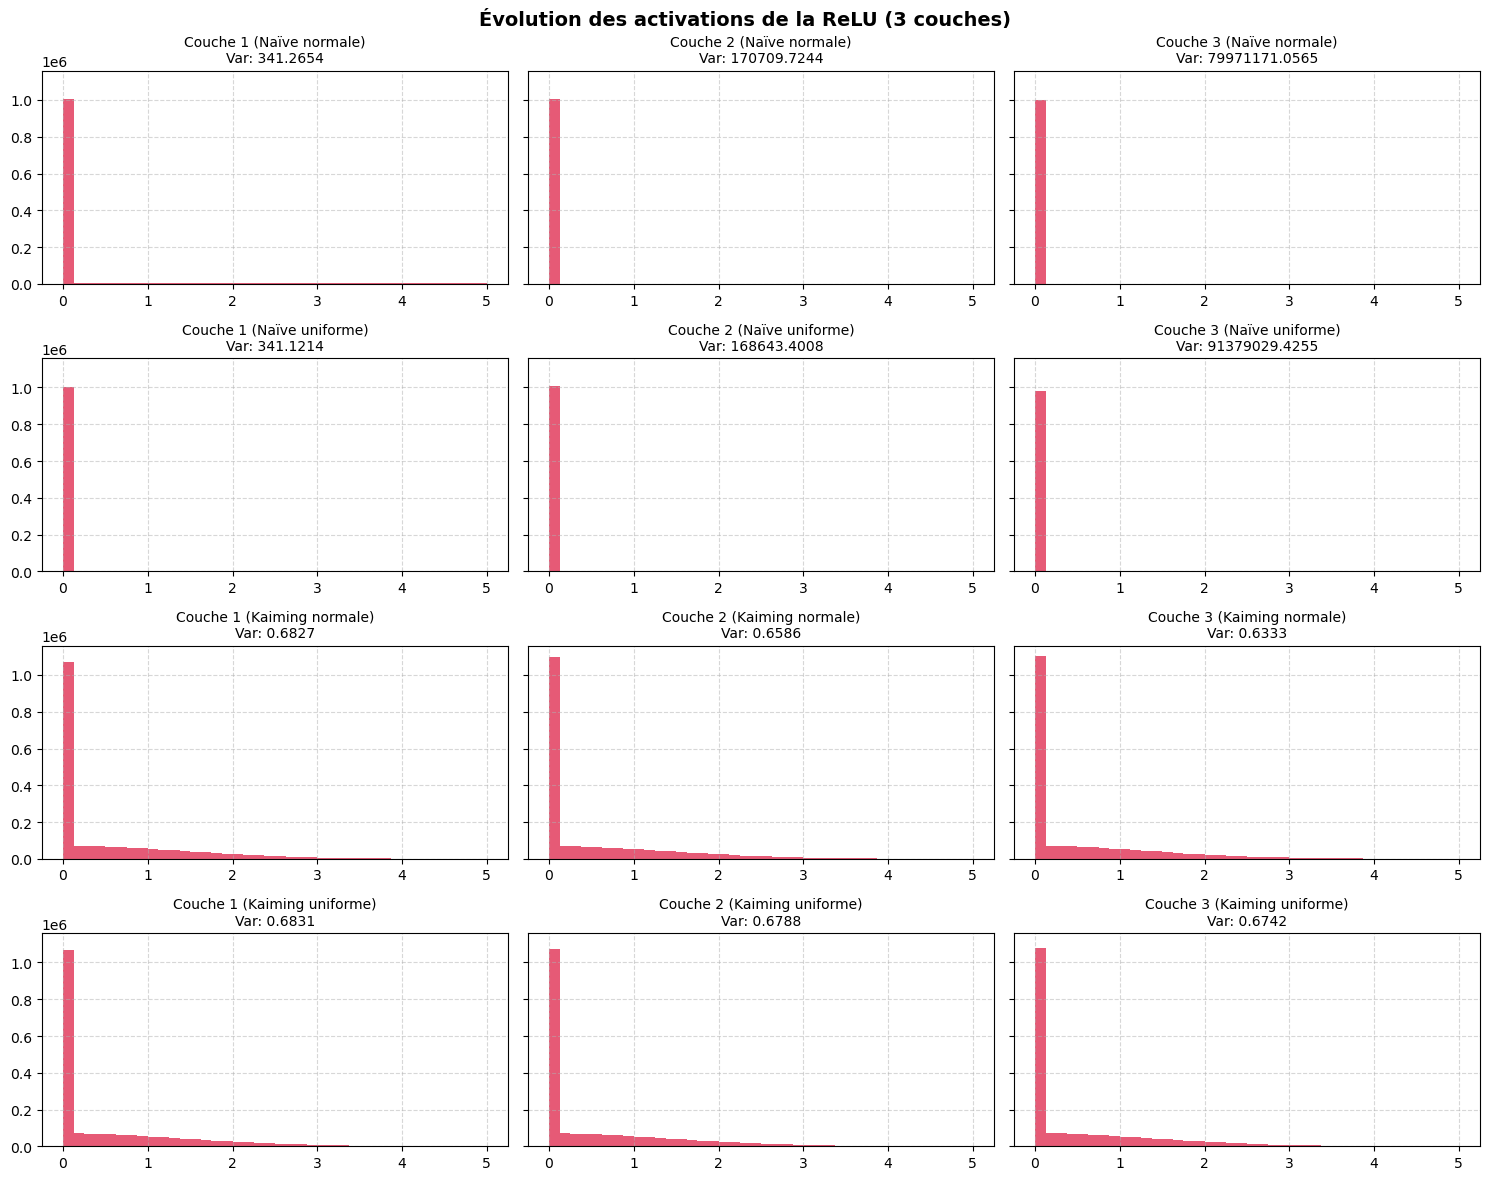
\includegraphics[width=1.0\linewidth]{Images/kaiming_relu}
				\label{fig:kaiming_relu}
			\end{figure}				
		\end{column}
		\begin{column}{0.35\textwidth}
			Avec une initialisation naïve des poids centrés en 0 et de variance unitaire, on observe une saturation pour 50\% des neurones et une explosion des valeurs pour les autres (la variance explose).
			
			\vspace{0.5cm}
			
			Avec l'initialisation de Kaiming (uniforme ou normale) nous observons une saturation attendue mais une variance qui reste stable au passage des différentes couches.
		\end{column}
	\end{columns}
\end{frame}

\begin{frame}{Conclusions sur les initialisations}
	Une bonne initialisation des poids est nécessaire pour prévenir les explosions ou disparitions de gradients au début de l'apprentissage d'un réseau de neurones mais ne garantit pas à elle seule que les gradients n'exploseront ou ne disparaîtront jamais.
	
	\pause
	\vspace{0.5cm}
	
	Les techniques d'initialisation des poids sont aussi combinées à un choix judicieux de la fonction d'activation (ReLU pour les réseaux profonds) et à d'autres techniques dont nous n'avons pas discuté comme la normalisation par batch, très utilisée sur les réseaux profonds. Certaines architectures de réseaux profonds sont spécialement conçues pour permettre une grande profondeur (1000 couches) sans disparition de gradient: les residual networks.
	
	\pause
	\vspace{0.5cm}
	
	Nous n'avons pas discuté de l'initialisation des termes de biais car ces derniers sont simplement initialisés à 0 la plupart du temps.
\end{frame}

\subsection[Conclusions]{Conclusions}

\begin{frame}{Conclusions sur les fonctions de perte, les algorithmes d'optimisation et l'initialisation des paramètres}
	Dans cette section, nous avons passé en revue l'arsenal mathématique nécessaire pour la \textbf{mise à jour des paramètres} du réseau de neurones:
	\begin{itemize}
		\item Nous avons discuté des \textbf{fonctions de pertes} pour:
		\begin{itemize}
			\item Les problèmes de régression.
			\item Les problèmes de classification binaire.
			\item Les problèmes de classification multi-classe.
		\end{itemize}
		\item Nous avons également vu quelques techniques utilisées dans l'industrie pour accélérer les calculs de rétro-propagation en \textbf{combinant} les \textbf{fonctions d'activation} de la dernière couche avec la \textbf{fonction de perte} elle-même.
	\end{itemize}
\end{frame}


\begin{frame}{Conclusions sur les fonctions de perte, les algorithmes d'optimisation et l'initialisation des paramètres}
	\begin{itemize}
		\item Nous avons introduit 3 variantes de l'algorithme de la descente du gradient:
		\begin{itemize}
			\item La technique du \textbf{momentum} pour lisser la trajectoire.
			\item La technique du taux d'apprentissage \textbf{adaptatif} pour accélérer la convergence tout en préservant la stabilité numérique.
			\item La combinaison des deux techniques précédente qui donne accès un algorithme de référence pour les réseaux de neurones: \textbf{Adam}.
		\end{itemize}
		\item Enfin, nous avons vu comment \textbf{initialiser} les poids afin de prévenir les problèmes d'\textbf{explosion} ou de \textbf{disparition} du gradient dans les premiers instants de l'apprentissage.
	\end{itemize}
\end{frame}